
\usetikzlibrary{calc,angles,quotes}

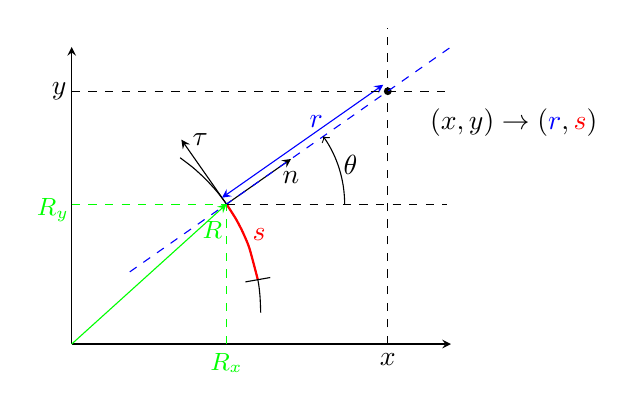
\begin{tikzpicture}[x={(0.8cm,0cm)}, y={(0cm,0.8cm)}, z={(-3.85mm, -3.85mm)}]%


\def\rayon{3}

%styledesnœuds
\tikzstyle{textLine}=[rectangle, text=black]
\tikzstyle{textw}=[rectangle, text=black]
\tikzstyle{pointx}=[circle, fill, scale=0.2]
\tikzstyle{vector}=[-stealth,thin]




%local normal base
\coordinate (p3) at (30:\rayon);
\coordinate (p4) at (35:\rayon);
\coordinate (p5) at (40:\rayon);
\coordinate (t) at ($(p4)!1cm!($(p4)+(p5)-(p3)$)$);
\coordinate[rotate around={-90:(p4)}] (n) at (t);


\def\sangle{10}
\coordinate(s0) at (\sangle:\rayon);

\def\coordListBefore{(0:\rayon) (5:\rayon) (10:\rayon) (20:\rayon) (25:\rayon) (27:\rayon)}
\def\coordList{(p3) (p4) (p5)}
\def\coordListAfter{(45:\rayon) (50:\rayon) (55:\rayon)}
\def\scoordList{(\sangle:\rayon)  (20:\rayon) (25:\rayon) (27:\rayon) (p3) (p4)}

%figure interface
\draw[black] plot[smooth, tension=0.4] coordinates {\coordListBefore \coordList \coordListAfter};

%figure base vectors
\draw[vector] (p4) -- (t);
\draw[vector] (p4) -- (n);
\node[textLine] (nn) at ($(n)+(0,-0.3)$) {$\boldsymbol{n}$};
\node[textLine] (tt) at ($(t)+(0.3,0)$) {$\boldsymbol{\tau}$};

%figure coord s
\draw[red,thick] plot [smooth, tension=0.4] coordinates {\scoordList};
\node[textLine,color=red] (ss) at ($($(s0)+(\sangle:0.3)$)!0.5!($(p4)+(35:0.3)$)$) {$s$};
\draw($(s0)-(\sangle:0.2)$) -- ($(s0)+(\sangle:0.2)$);

%figure point x
\coordinate (x) at ($(p4)!2.5!(n)$);

\node[pointx, scale=1.5] at (x) {};
\node[textLine,text centered] (chg) at ($(x)+(2,-0.5)$) { $(x,y)\rightarrow (\textcolor{blue}{r},\textcolor{red}{s})$};

%figure axis
\coordinate (oo) at (0,-0.5);%
\coordinate (ox) at ($(oo)+(1,0)$);%
\coordinate (oy) at ($(oo)+(0,1)$);%
\draw[vector] (oo) -- ($(oo)!($1.2*(x)$)!(ox)$);%
\draw[vector] (oo) -- ($(oo)!($1.2*(x)$)!(oy)$);%


%figure coord r
\draw[dashed,color=blue] ($(p4)!-1.5!(n)$) -- ($(x)-(p4)+(p4)!1!(n)$);%
\draw[stealth-stealth,thin,color=blue] ($($(p4)!0.1!(t)$)$) -- ($(x)-(p4)+($(p4)!0.1!(t)$)$);%
\node[textLine,color=blue] (rsize) at ($(n)+(0.4,0.6)$) {$r$};%

% projection cartesian xy
\draw[dashed] ($(oo)!(x)!(oy)$) -- ($(x)+(1,0)$);%
\draw[dashed] ($(oo)!(x)!(ox)$) -- ($(x)+(0,1)$);%
\node[textLine] at ($(oo)+($(oo)!(x)!(ox)$)+(0,0.25)$) { $x$};%
\node[textLine] at ($(oo)+($(oo)!(x)!(oy)$)+(-0.2,0.5)$) { $y$};%

%figure theta
\draw[dashed] ($(p4)$) -- ($(p4)+(3.5,0)$);%
\coordinate (p4x) at ($(p4)+(1,0)$);%

\pic[draw,->, "$\theta$", angle eccentricity=1.1, angle radius=1.5cm] {angle=p4x--p4--n};
% PROBLEM HERE !!!! at "$\theta$" -> SOLVED = missing "quotes" tikzlibrary

%figure R
\draw[vector,color=green] (oo) -- (p4);%
\node[textLine,color=green] (Rtext) at ($(oo)!0.95!(p4)-(0.1,0.3)$) {\small$\boldsymbol{R}$};%
\draw[dashed,color=green] ($(oo)!(p4)!(oy)$) -- ($(p4)$);%
\draw[dashed,color=green] ($(oo)!(p4)!(ox)$) -- ($(p4)$);%
\node[textLine,color=green] at ($(oo)+($(oo)!(p4)!(ox)$)+(0,0.2)$) {\small$R_x$};%
\node[textLine,color=green] at ($(oo)+($(oo)!(p4)!(oy)$)-(0.3,-0.4)$) {\small$R_y$};%


\end{tikzpicture}
